\documentclass[a4paper,11pt,fleqn]{article}%fleqn pour aligner les equations à gauche
\usepackage{graphicx}
\usepackage[utf8]{inputenc}  
\usepackage[T1]{fontenc}
\usepackage{lscape}

\usepackage{tgheros,textcomp}%Police Arial
\renewcommand{\familydefault}{\sfdefault}

%\setlength{\mathindent}{0pt}%indentation dans math = 0

\usepackage[top = 1cm, bottom = 2cm, left = 1cm, right = 1cm]{geometry}
\usepackage{titlesec}
%\setcounter{secnumdepth}{4}
\usepackage{xcolor}
\usepackage{amssymb} %double flèche de réaction
\usepackage{mathrsfs}%farraday
\usepackage{xtab}%tableau sur plusieurs pages
\usepackage{esvect}%grands vecteurs

\usepackage[version=4]{mhchem} %equations chimiques

\usepackage{array}
\usepackage{chemfig}
\usepackage{multirow}
%\usepackage{sectsty}

\usepackage{caption}
\usepackage{adjustbox}
\usepackage[labelformat=simple]{subfig}
\usepackage{float}


\usepackage{amsmath}
\usepackage{amssymb}
\usepackage[cal=boondoxo]{mathalfa} 
\usepackage{enumitem}
\usepackage{lastpage}
\usepackage{tcolorbox}
\usepackage{siunitx}
\usepackage[european, straightvoltages, RPvoltages]{circuitikz}
\usepackage{tikz}
\usetikzlibrary{shapes.geometric}
\usetikzlibrary{calc}
\usetikzlibrary{automata,positioning}
\usepackage{multicol}
\usepackage{eqnarray}
\usepackage{tabularx,colortbl}%colorer fond cellules

\sisetup{
	detect-all,
	output-decimal-marker={,},
	group-minimum-digits = 3,
	group-separator={~},
	number-unit-separator={~},
	inter-unit-product={~}
} %setup pour SIunitx

\usepackage{listings}%pour insérer le code python
\definecolor{codegreen}{rgb}{0,0.6,0}
\definecolor{codegray}{rgb}{0.5,0.5,0.5}
\definecolor{codepurple}{rgb}{0.58,0,0.82}
\definecolor{backcolour}{rgb}{0.95,0.95,0.92}


\titleformat{\section}
{
\vspace{.8ex}%
\normalfont \bfseries \large}
{\thesection.}{.5em}{\bfseries}

\renewcommand{\thesection}{\arabic{section}}
\titlespacing{\section}{0pt}{.5em}{.5em}
\renewcommand{\thesubsection}{\hspace{1cm}\alph{subsection}.}
\renewcommand\thesubfigure{\textbf{Document \arabic{subfigure} :}}

\title{\vspace{-1cm}\noindent\large 
	\centering \begin{tabular}{|>{\centering}m{5cm}|>{\centering}m{8cm}|>{\centering\arraybackslash}m{4cm}|}
		\hline
		Activité 3 & \textbf{\textsc{Mesure de la longueur du méridien terrestre par Delambre et Méchain}} &  Chapitre 4 \\
		\hline
\end{tabular}}
\date{}

\newpagestyle{mystyle}{%
	\setfoot{}{\thepage\,$|$\,\pageref{LastPage}}{}
}
\renewpagestyle{plain}{%
	\setfoot{}{\thepage\,$|$\,\pageref{LastPage}}{}
}

\pagestyle{mystyle}

\newenvironment{itemize*}%
{\begin{itemize}[label=$-$,topsep=0pt]%
		\setlength{\itemsep}{0pt}%
		\setlength{\parskip}{0pt}}%
	{\end{itemize}}

\newenvironment{itemize**}%
{\begin{itemize}[label=,labelindent=0pt, leftmargin=*,topsep=0pt]%
		\setlength{\itemsep}{0pt}%
		\setlength{\parskip}{0pt}}%
	{\end{itemize}}

\renewcommand{\arraystretch}{1.5}


\begin{document}
\maketitle
\vspace{-2cm}

Suite à la Révolution française, s'est imposé la révolution métrique ! En effet, chaque pays, chaque région de France, possédait jusqu'alors ses propres unités de mesure, rendant les échanges commerciaux compliqués. \textbf{Quelle est la définition historique du mètre ? En quoi consiste la méthode de triangulation utilisée par Delambre et Méchain ?}\\

\noindent \colorbox{blue!10}{\begin{minipage}{.5\linewidth}
		\textcolor{purple!30!blue}{\textbf{Document 1 : Première définition du mètre}}\\
		\begin{minipage}{.65\textwidth}
        En 1970, l'Assemblée nationale française décide d'établir un système de mesure unique. il faut une mesure "pour tous les temps et pour tous les peuples". De nombreux savants sont associés à ce projet. La Terre est alors choisie comme référence et le mètre défini comme la dix millionième partie du quart  du méridien terrestre. Mais il faut en faire la mesure puisque précisément le mètre n'existe pas encore ! C'est à Pierre Méchain (1744-1804) et Jean-Baptiste Delambre (1749-1822), astronomes et mathématiciens, qu'est confiée la mission d'effectuer des premières mesures qui débutent en 1792.
        \end{minipage}
        \begin{minipage}{.3\textwidth}
            \begin{center}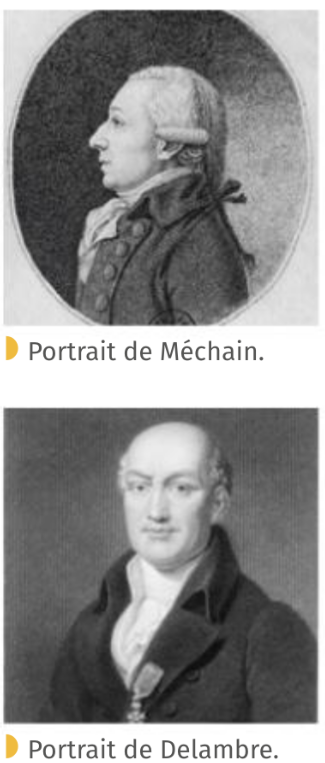
\includegraphics[scale=.3]{Ressources/1ES_C4_AE3_Fig2.png}\end{center}
        \end{minipage}
\end{minipage}}
\colorbox{blue!10}{\begin{minipage}{.5\linewidth}
		\textcolor{purple!30!blue}{\textbf{Document 2 : La moitié Nord du méridien de Paris}}
		\begin{center}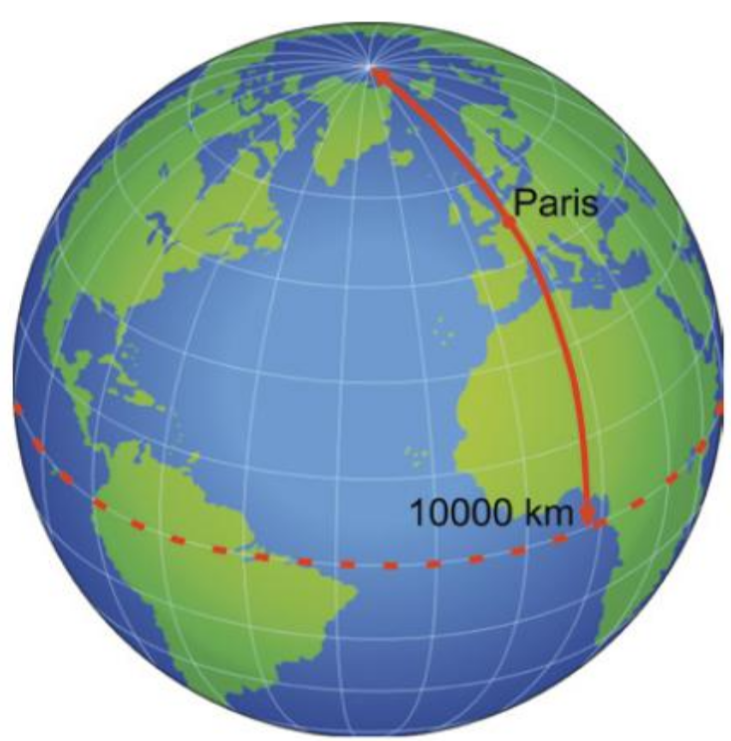
\includegraphics[scale=.31]{Ressources/1ES_C4_AE3_Fig1.png}\end{center}
\end{minipage}}
\vspace{.2cm}

\noindent \colorbox{blue!10}{\begin{minipage}{\linewidth}
		\textcolor{purple!30!blue}{\textbf{Document 3 : Mesure du méridien par Delambre et Méchain}}\\
		Delambre et Méchain mesurent avec précision la longueur d'une portion du méridien terrestre passant par Dunkerque, Paris et Barcelone, en toises, unité de l'époque. Ils partent chacun de Paris dans des directions opposées. C'est par une succession de mesures d'angles qu'ils parviennent à mesurer la distance Dunkerque-Barcelone puis ensuite l'arc de méridien entre ces deux villes. Leurs résultats donnent alors une valeur du mètre fixée à \num{0,513074} toise.\\
        Ils rencontrent de nombreuses difficultés, car la période (Terreur) n'est pas propice aux déplacements avec un appareil de mesure inhabituel, un cercle répétiteur (un pied pour des mesures à hauteur d'homme, un cercle gradué et deux lunettes de visée).\\
        Delambre rencontre des problèmes avec des gardes nationaux, peu coopératifs et intéressés. Pendant une année, il ne peut pas travailler. Méchain a plus de chance au début mais en 1793, l'Espagne déclare la guerre à la France et ses mesures deviennent plus compliquées à réaliser. Il constate au final une anomalie de quelques secondes d'arc qui le poussa à cacher ses mesures.
\end{minipage}}
\vspace{.2cm}

\noindent \colorbox{orange!10}{
\begin{minipage}{.5\linewidth}
    \textbf{Maths !}\\
Dans un triangle ABC tel que la figure ci-contre, on a : $$ \dfrac{a}{\sin{\widehat{A}}} = \dfrac{b}{\sin{\widehat{B}}} = \dfrac{c}{\sin{\widehat{C}}} $$
\end{minipage}
\begin{minipage}{.5\linewidth}
    \centering
    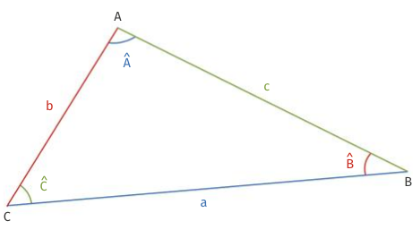
\includegraphics[scale=.5]{Ressources/1ES_C4_AE3_Fig6.png}
\end{minipage}}

\noindent \colorbox{blue!10}{
\begin{minipage}{.6\linewidth}
		\textcolor{purple!30!blue}{\textbf{Document 4 : Méthode de mesure par triangulation}}\\
		La méthode consiste à mesurer précisément une base $AB$. La base est alors l'origine d'une opération de triangulation. À partir des extrémités $A$ et $B$ de cette base. Delambre et Méchain visent un point $C$ éloigné et mesurent les angles $\widehat{CAB}$ et $\widehat{CBA}$. Ils en déduisent la distance $BC$ en utilisant les relations du triangle. Celle-ci constitue alors la base d'un nouveau triangle dont le sommet est $D$.

        \begin{center}
            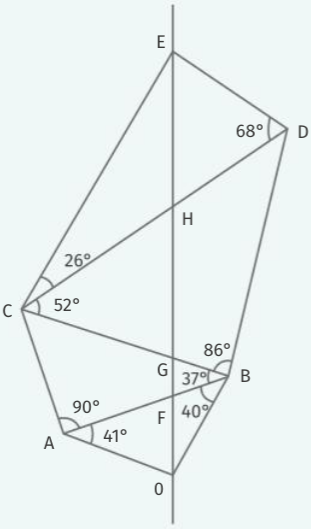
\includegraphics[scale=.6]{Ressources/1ES_C4_AE3_Fig4.png.png}
        \end{center}
\end{minipage}
\begin{minipage}{.4\linewidth}
        \centering
        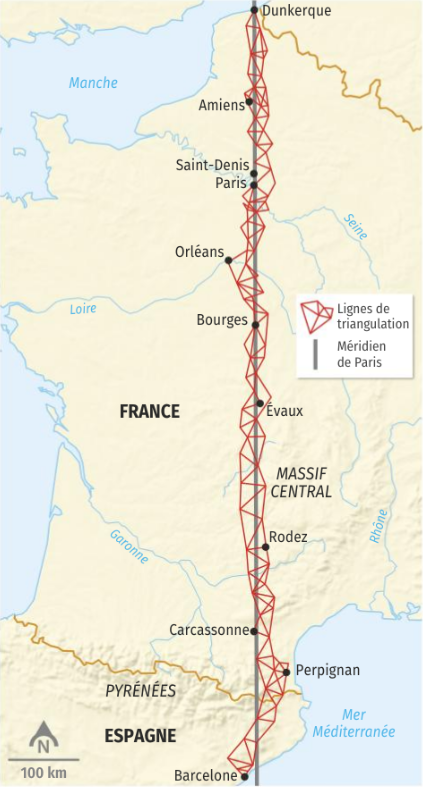
\includegraphics[scale=.5]{Ressources/1ES_C4_AE3_Fig5.png.png}
\end{minipage}}

\subsection*{Questions :}
\begin{enumerate}
    \item \textcolor{orange}{\textbf{Doc. 1}} Dans quel contexte historique se trouvait la France à l'époque de Delambre et Méchain ?
    \item \textcolor{orange}{\textbf{Doc. 1}} Pourquoi a-t-il été indispensable de fixer des unités de mesure communes à tous les pays en donnant naissance à un "système international" ?
    \item \textcolor{orange}{\textbf{Doc. 1}} Quelle référence incontestable a-t-on choisie pour définir l'unité internationale de longueur, le mètre ?
    \item \textcolor{orange}{\textbf{Doc. 3 et 4}} Quel protocole expérimental ont été utilisé Delambre et Méchain pour mesurer la distance Dunkerque-Barcelone ?
    \item \textcolor{orange}{\textbf{Doc. 4}} À l'aide de la carte, évaluer cette distance en mètre et en toises.
    \item \textcolor{orange}{\textbf{Doc. 3 et 4}} Énoncez et commentez les problèmes qu'ont rencontrés Delambre et Méchain.
    \item \textcolor{orange}{\textbf{TP}} Sur le schéma, sachant que l'on connaît la distance $AB$ = \SI{11}{km}, que les angles déterminés par triangulation sont indiqués et les angles manquants à mesure avec un rapporteur, calculez la longueur $OE$ représentant une portion de méridien.
    \item Le Bureau international des poids et mesures, organisation intergouvernementale dont les États membres agissent en commun concernant les sujets liés à la science des mesures et leurs étalons, a fait évoluer la définition du mètre. Effectuer des recherches pour déterminer la définition actuelle du mètre.
\end{enumerate}

\end{document}
\begin{tikzpicture}[scale=.5]
	\node[below right] (O)at (0,0) {O};
	\node[left] (A) at (-6.683,2.565) {A};
	\node[right] (B) at (3.653,6.328) {B};
 
    \node[left] (C) at (-8.257,10.703) {C};
    \node[right] (D) at (10.198,19.704) {D};
    \node[above left] (E) at (3.483,25.741) {E};
 
    \draw (-6.675,2.566) -- (3.868,6.699) -- (0,0) -- cycle;
    \draw (-6.675,2.566) -- (-8.257,10.703) --(3.868,6.699);
    \draw (3.868,6.699) -- (10.198,19.704) -- (-8.257,10.703);
    \draw (10.198,19.704) -- (3.483,25.741) -- (-8.257,10.703);
    \draw (0,0) -- (0,25.741);
			
	%\draw (2.65,-.5) arc(-80:0:.5);
	%\draw (2.4,-1.5) arc(80:180:.5);
\end{tikzpicture}